\title{Error Analysis in PHYS180}
\author{Jordan C. Hanson}
\date{\today}
\documentclass[12pt]{article}
\usepackage[margin=2cm]{geometry}
\usepackage{amsmath,mathtools}
\usepackage{graphicx}

\begin{document}
\maketitle

\begin{abstract}
Scientific measurements cannot be quoted without an assessment of the precision.  We quantify this precision in the form of error analysis.  Rather than originating from \textit{human error}, \textit{statistical errors} arrise from the intrinsic uncertainty encounted in measuring quantities with real instruments.  Further, errors \textit{propagate} through calculations.  This document will explain how this works, and how to perform error analysis for final results.
\end{abstract}

\section{Instrumental Precision}

The instrumental precision of a piece of data is determined by the smallest division on the instrument.  For example, suppose a length is measured with a meter stick, and the smallest divisions on the meter stick are 1 millimeter.  If the length measured is 31.0 cm, then that result must be stated as $31.0\pm0.1$ cm.

\section{Accuracy versus Precision}

Accuracy and precision are not the same concept.  Accuracy is how far the measured result is from the true value, whereas precision compares the statistical error of a measurement to the measured value itself.  A measurement of $31.0\pm0.1$ cm is precise, because 0.1 cm is small compared to 31.0 cm.  It is not \textit{accurate} if the true length is 29.0 cm.  Why? Because the numbers 31.0 cm and 29.0 cm are separated by $(31.0-29.0)/0.1 = 20$ factors of the error.

\section{Statistical or Random Error}

Suppose a measurement is made with a dial, where a needle is pointing to a number, but vibrating.  When the dial is read one moment, it reads $101.3$ kPa, and in another moment, $101.2$ kPa.  Which pressure measurement of the atmosphere is correct?  It turns out that upon repeated measurements, the \textit{distribution} of measurements resembles Fig. \ref{fig:histo}.

\begin{figure}
\centering
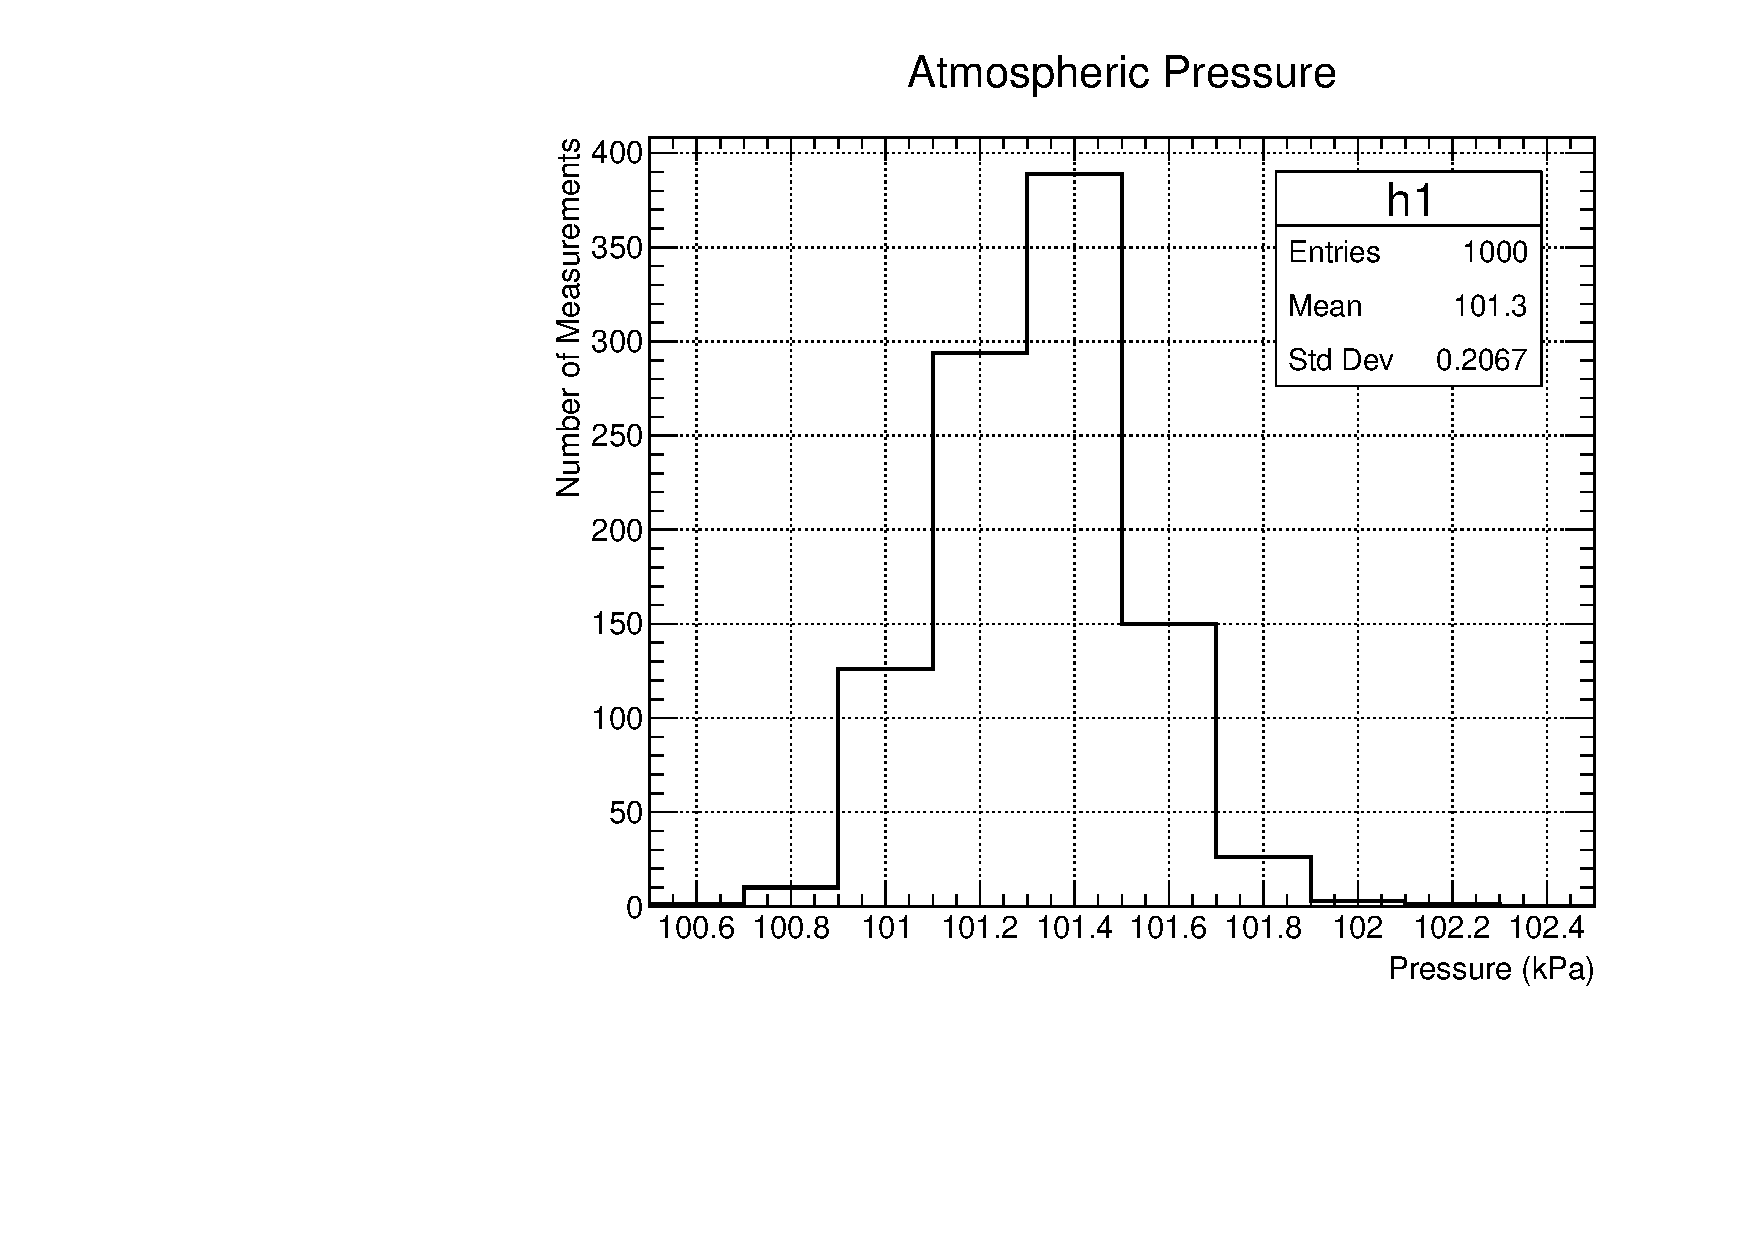
\includegraphics[width=0.5\textwidth]{histo.pdf}
\caption{\label{fig:histo} An example of a distribution of measurements from one instrument: a pressure gauge.}
\end{figure}

It's not that there isn't a true pressure, there is, and it is most likely 101.3 kPa.  In reality, the dial needle is moving, making identification of the \textit{exact} or true pressure impossible.  Instead, the true value is ascertained from the statistical distribution.

\section{Analysis of Data Subject to Random Error}

It turns out that computing the standard deviation of several measurements and the mean of those measurements is an altogether \textit{different} question than computing the errors \textit{in each measurement}, if the measurement is made from combining other measured quantities.  For example, suppose the latent heat of water is measured by 

\end{document}
